%%%%%%%%%%%%%%%%%%%%%%%%%%%%%%%%%%%%%%%%%%%%%%%%%%%%%%%%%%%%%%%%%%%%%%%%%%%%%%%%
%2345678901234567890123456789012345678901234567890123456789012345678901234567890
%        1         2         3         4         5         6         7         8

\documentclass[letterpaper, 10 pt, conference]{ieeeconf}  % Comment this line out
                                                          % if you need a4paper
%\documentclass[a4paper, 10pt, conference]{ieeeconf}      % Use this line for a4
                                                          % paper

\IEEEoverridecommandlockouts                              % This command is only
                                                          % needed if you want to
                                                          % use the \thanks command
\overrideIEEEmargins
% See the \addtolength command later in the file to balance the column lengths
% on the last page of the document

\usepackage[utf8]{inputenc}
\usepackage[T1]{fontenc}

% The following packages can be found on http:\\www.ctan.org
\usepackage{graphicx} % for pdf, bitmapped graphics files
%\usepackage{epsfig} % for postscript graphics files
%\usepackage{mathptmx} % assumes new font selection scheme installed
%\usepackage{mathptmx} % assumes new font selection scheme installed
\usepackage{amsmath} % assumes amsmath package installed
%\usepackage{amssymb}  % assumes amsmath package installed

\title{\LARGE \bf
Lab2: Position control and Dynamics
}

%\author{ \parbox{3 in}{\centering Huibert Kwakernaak*
%         \thanks{*Use the $\backslash$thanks command to put information here}\\
%         Faculty of Electrical Engineering, Mathematics and Computer Science\\
%         University of Twente\\
%         7500 AE Enschede, The Netherlands\\
%         {\tt\small h.kwakernaak@autsubmit.com}}
%         \hspace*{ 0.5 in}
%         \parbox{3 in}{ \centering Pradeep Misra**
%         \thanks{**The footnote marks may be inserted manually}\\
%        Department of Electrical Engineering \\
%         Wright State University\\
%         Dayton, OH 45435, USA\\
%         {\tt\small pmisra@cs.wright.edu}}
%}

\author{Yiwen(Robert) Wu\\\\https://github.com/Robert1124/cse460}


\begin{document}



\maketitle
\thispagestyle{empty}
\pagestyle{empty}

\section{Exercise 5}

The P-controller was implemented in accordance with the control law given by:

\begin{equation}
    u(t) = K (\mathbf{p}_d - \mathbf{p}(t)),
    \label{eq:p_control_law}
\end{equation}

where \( K \) is the proportional gain, \( \mathbf{p}_d \) is the desired position vector, and \( \mathbf{p}(t) \) is the current position vector of the robot at time \( t \). This control law computes the control input \( u(t) \) as a function of the instantaneous error between the desired and current positions.

A discrete-time simulation was conducted over a time frame of 20 seconds with a time step of 0.01 seconds. At each time step, the control input was calculated and applied to update the robot's position using the Euler method for numerical integration. The proportional gain was set to \( K = 1.0 \).

The position update was defined as:

\begin{equation}
    \mathbf{p}(t + \Delta t) = \mathbf{p}(t) + \Delta t \cdot u(t),
    \label{eq:euler_integration}
\end{equation}

where \( \Delta t \) is the time step, and \( u(t) \) is the control input from Equation \ref{eq:p_control_law}.

The robot's trajectory was plotted, showing its progression from the initial to the desired location. The plot demonstrated the effectiveness of the P-controller in guiding the robot along a straight path towards the target.

The implemented P-controller successfully directed the robot to the desired location. The simplicity of the P-control strategy made it straightforward to apply and effective for this scenario. However, it is important to note that the selection of the proportional gain \( K \) can significantly affect the controller's performance, potentially leading to overshoot or oscillations if not chosen appropriately.

\begin{figure}[htbp]
    \centering
    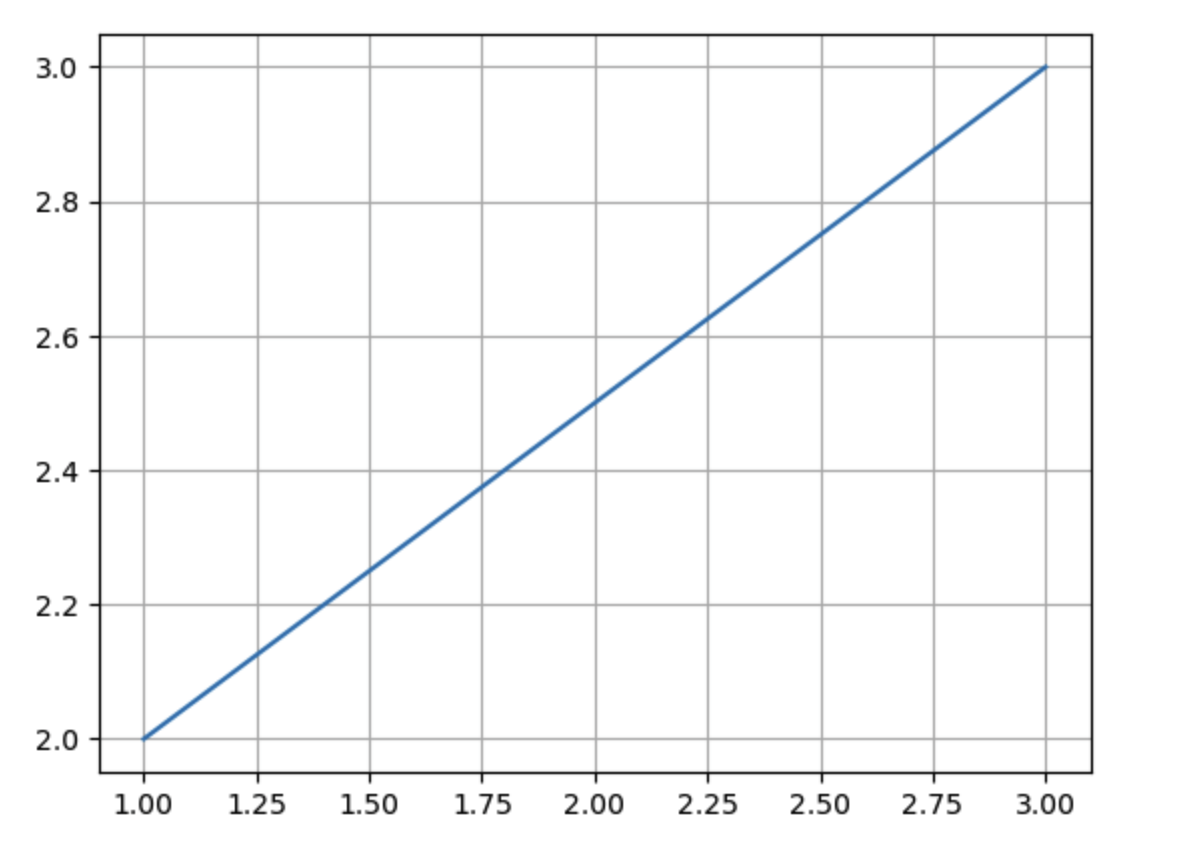
\includegraphics[width=0.4\textwidth]{image1.png}
\end{figure}

\section{Exercise 6}

A robotic agent was tasked to navigate a complex zigzag trajectory using a Proportional (P) controller, which bases the control input on the positional error. The P-controller was defined by the equation \( u(t) = K (\mathbf{p}_d - \mathbf{p}(t)) \), where \( K \) is the proportional gain, \( \mathbf{p}_d \) is the target position, and \( \mathbf{p}(t) \) is the current position of the robot. The controller's efficacy was determined by its ability to steer the robot accurately through each waypoint on the zigzag path.

The waypoints were carefully chosen to represent the corners of the zigzag path, which the robot was to follow. Starting from an initial location of \( [-3, -3]^\top \), the robot was directed towards each waypoint successively, with the control input updated at a fixed time step of 0.01 seconds. For this task, the proportional gain was set to 1.0, balancing the system's responsiveness against stability.

During the simulation, which lasted for 20 seconds, the robot's position was updated using the Euler method. This numerical integration approach allowed for a straightforward and computationally efficient means of simulating the robot's trajectory. As the robot progressed along the path, its position at each time step was recorded, creating a log of its journey.

The plotted trajectory revealed that the robot was capable of closely following the desired path. The sharp turns at the waypoints were navigated with precision, and the control inputs successfully corrected the robot's course, ensuring it remained close to the intended route. The robot's path, as visualized in the plot, confirmed the robustness of the P-controller in guiding the robot along the specified zigzag pattern.

\begin{figure}[htbp]
    \centering
    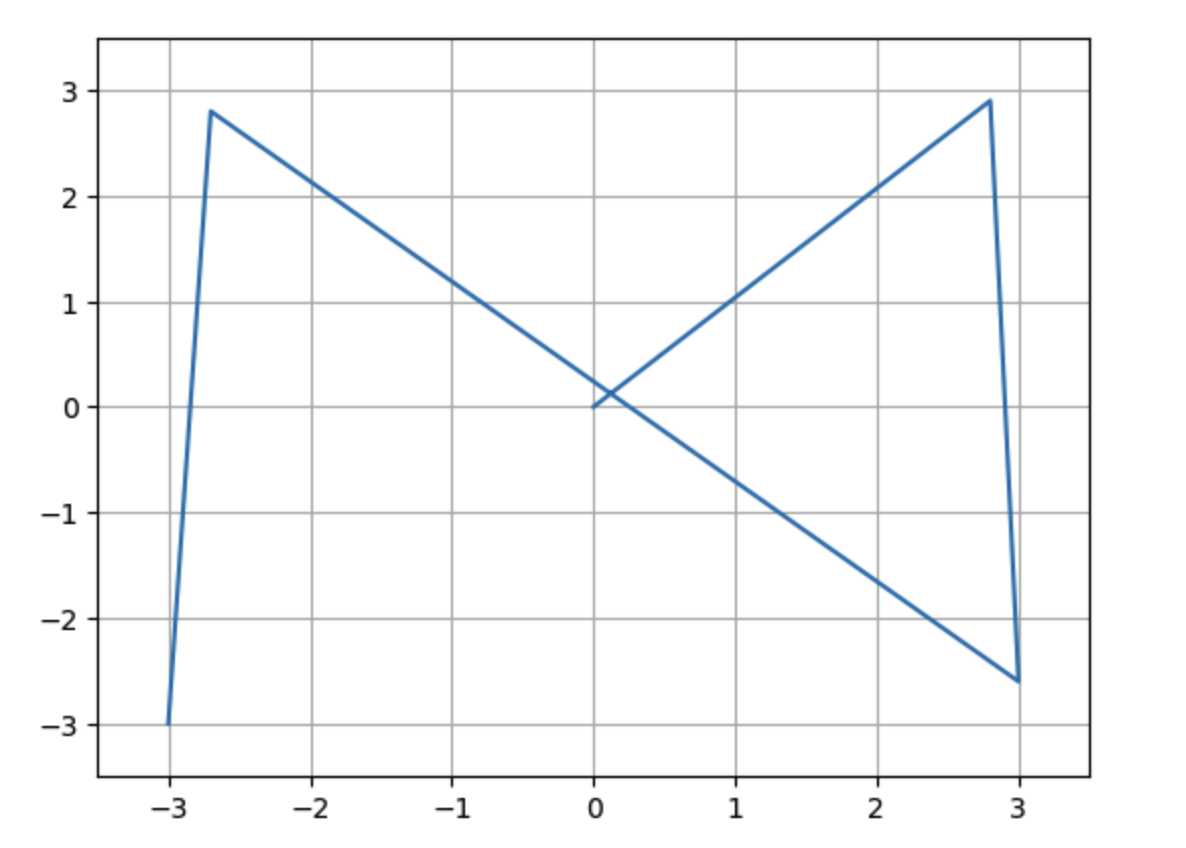
\includegraphics[width=0.5\textwidth]{image2.png}
\end{figure}

\section{Part2-1 Free Fall}
In the study of robotic motion, simulating free fall is crucial for understanding the effects of gravitational forces on translational dynamics. The simulation of free fall involves creating a model that accurately represents the motion of a falling object under the influence of gravity alone. To this end, a simulator was developed to replicate the translational dynamics that an object experiences during free fall.

The translational dynamics are governed by Newton's second law of motion, which states that the force on an object is equal to the mass of the object multiplied by its acceleration (\( F = ma \)). In the case of free fall, the only force acting upon the object is the force of gravity, which can be expressed as \( F_g = mg \), where \( m \) is the mass of the object and \( g \) is the acceleration due to gravity. This force results in a downward acceleration of the object.

The simulator uses these principles to update the position and velocity of the object at each timestep. The equations of motion for the simulator are given by:

\begin{align*}
v(t+\Delta t) &= v(t) + g\Delta t, \\
p(t+\Delta t) &= p(t) + v(t)\Delta t + \frac{1}{2}g(\Delta t)^2,
\end{align*}

where \( v(t) \) is the velocity of the object at time \( t \), \( p(t) \) is the position of the object at time \( t \), \( g \) is the gravitational acceleration, and \( \Delta t \) is the timestep increment. The simulator iteratively applies these equations to calculate the position and velocity of the object as it falls freely under the influence of gravity.

Through this simulation, the object is observed to accelerate downwards, with its velocity increasing linearly over time, and its position changing according to the equations of motion for constant acceleration. This simulation not only reinforces fundamental physics concepts but also provides a basis for more complex simulations that may include additional forces, such as drag or lift, which are encountered by robotic systems in real-world scenarios.

\begin{figure}[htbp]
    \centering
    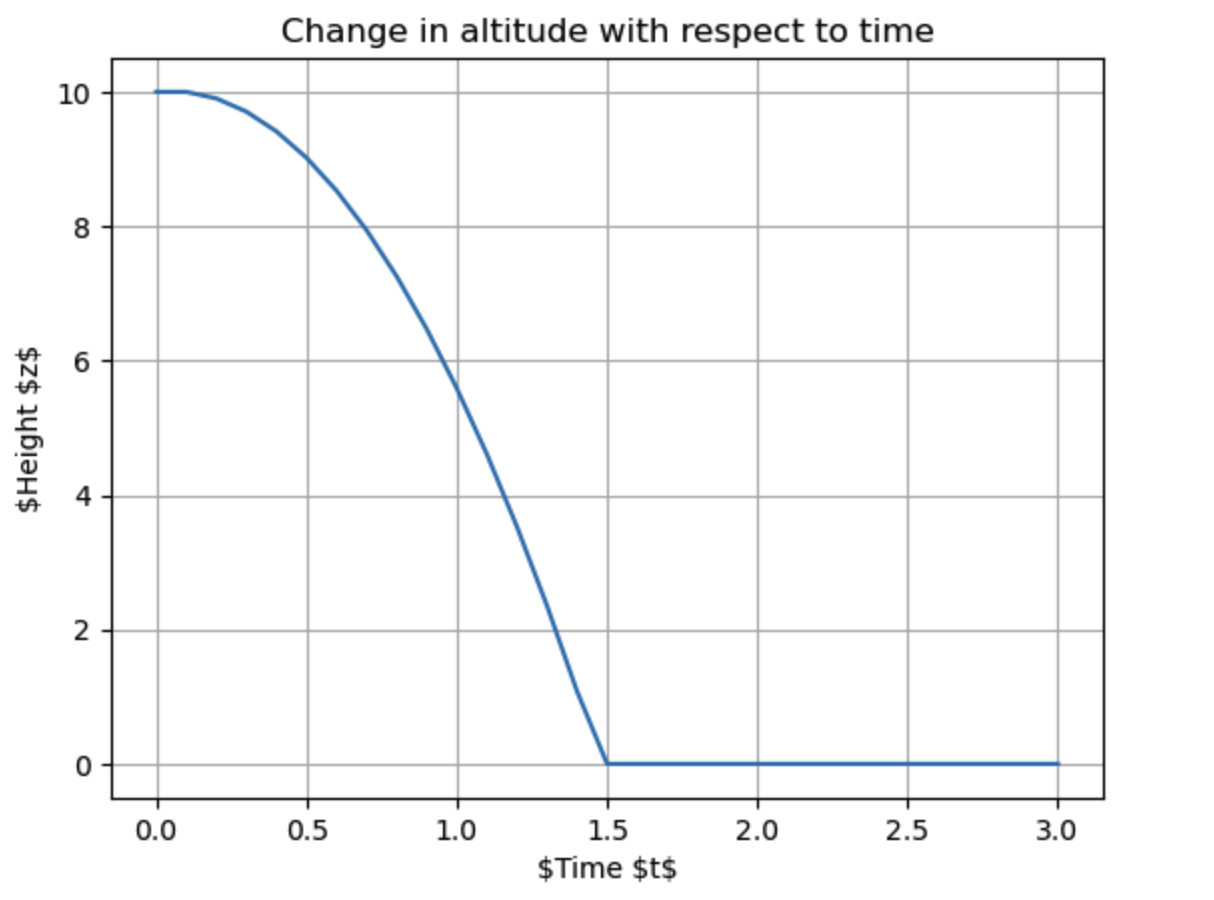
\includegraphics[width=0.5\textwidth]{image3.png}
\end{figure}

\section{Part2-2 fb=9.0}

The dynamics of an LTA vehicle, such as a helium balloon, were simulated to include the effects of buoyancy alongside gravity. This is crucial for applications where the vehicle operates in a fluid medium and experiences an upward buoyant force that opposes the weight of the vehicle. The simulation models the translational dynamics with the state vector being updated to account for buoyancy, gravity, and the lack of any other control inputs in the vertical direction.

Euler integration is employed to discretely update the state vector, consisting of position and velocity, at each time step. The buoyancy force is set to a constant value, reflecting the lift provided by the helium, while the simulation accounts for gravitational acceleration. The update rule for the vertical acceleration now includes the effects of buoyancy and is given by \( \ddot{z}(t) = \frac{u_z(t) + F_b - m \cdot g}{m} \), where \( F_b \) is the buoyancy force. A conditional statement simulates the impact with the ground, ensuring that the vehicle does not penetrate the surface, akin to a plastic collision.

In this simulation scenario, the buoyancy force is substantial enough to slow the vehicle's descent compared to free fall. The plot, illustrating the change in altitude with respect to time, depicts a trajectory that is less steep than that of an object in free fall, indicating a reduced rate of descent due to buoyancy. This contrast highlights the significance of buoyancy in modifying the dynamics of bodies within fluid environments.


\begin{figure}[htbp]
    \centering
    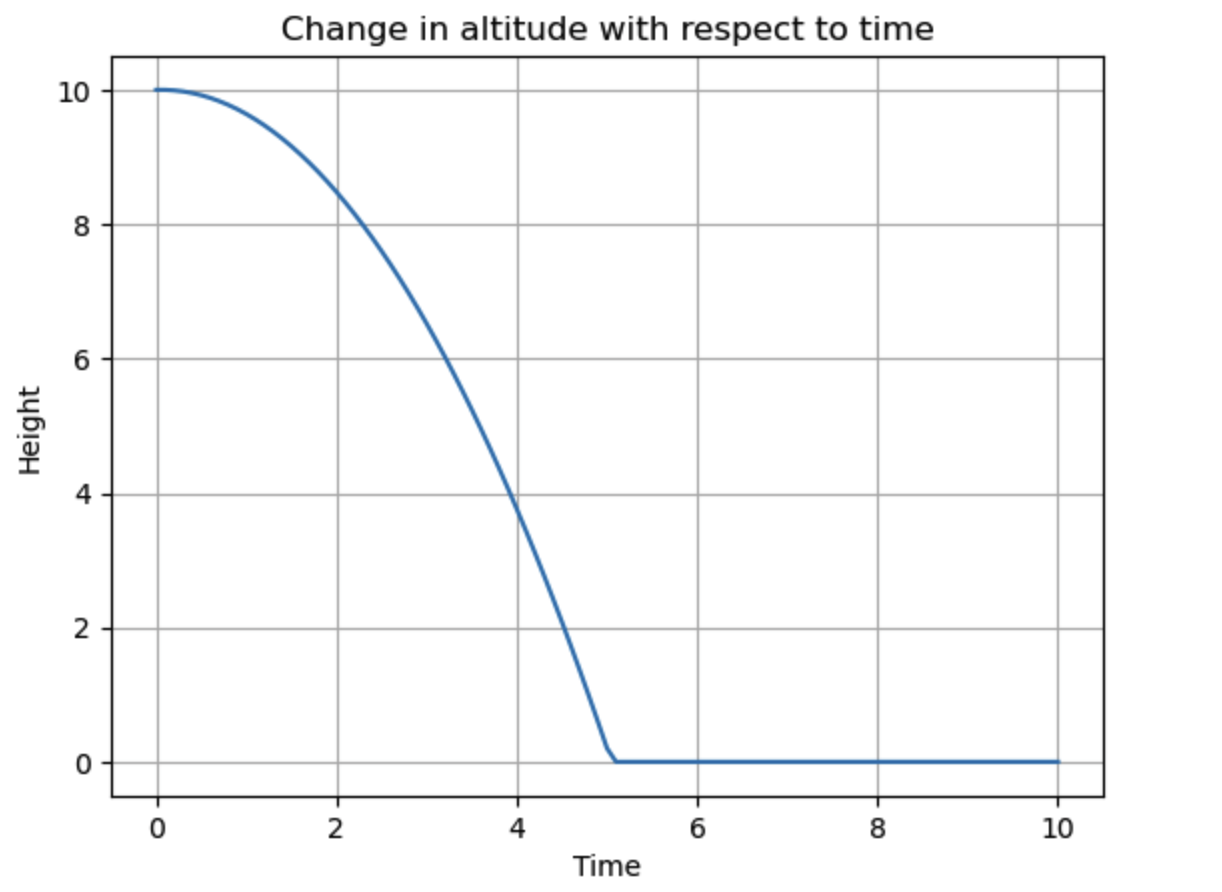
\includegraphics[width=0.5\textwidth]{image4.png}
\end{figure}

\section{Part2-4 Mass Mismatch}
A PD (Proportional-Derivative) controller was implemented to regulate the height of a robot within a simulated environment. The controller's goal was to adjust the robot's altitude to reach and maintain a desired height, compensating for gravitational forces. The control law for the PD controller is given by the equation:

\[ u(t) = K_p (z_d - z(t)) - K_d \frac{dz(t)}{dt}, \]

where \( u(t) \) is the control input at time \( t \), \( K_p \) is the proportional gain, \( K_d \) is the derivative gain, \( z_d \) is the desired height, \( z(t) \) is the current height, and \( \frac{dz(t)}{dt} \) is the derivative of the height with respect to time, representing the vertical velocity of the robot.

In the provided solution, the PD controller parameters were set with a proportional gain \( K_p = 2.0 \) and a derivative gain \( K_d = 1.0 \), with the aim of achieving a smooth and stable convergence to the desired height of \( z_d = 15 \) meters. The initial condition for the simulation placed the robot at a height of 10 meters, and the control input was updated at each time step to drive the robot towards the setpoint.

The simulation results, plotted over a period of 3 seconds, show the trajectory of the robot's height as it responds to the control input. The plot illustrates the robot's ascent towards the desired height, the effect of the PD controller in stabilizing the height, and the eventual descent as the robot overshoots the target height slightly due to momentum before settling at the desired altitude.

This PD controller's behavior demonstrates the typical response of such systems, where the proportional term reduces the error and the derivative term mitigates the velocity, contributing to a controlled and stable system response.

\begin{figure}[htbp]
    \centering
    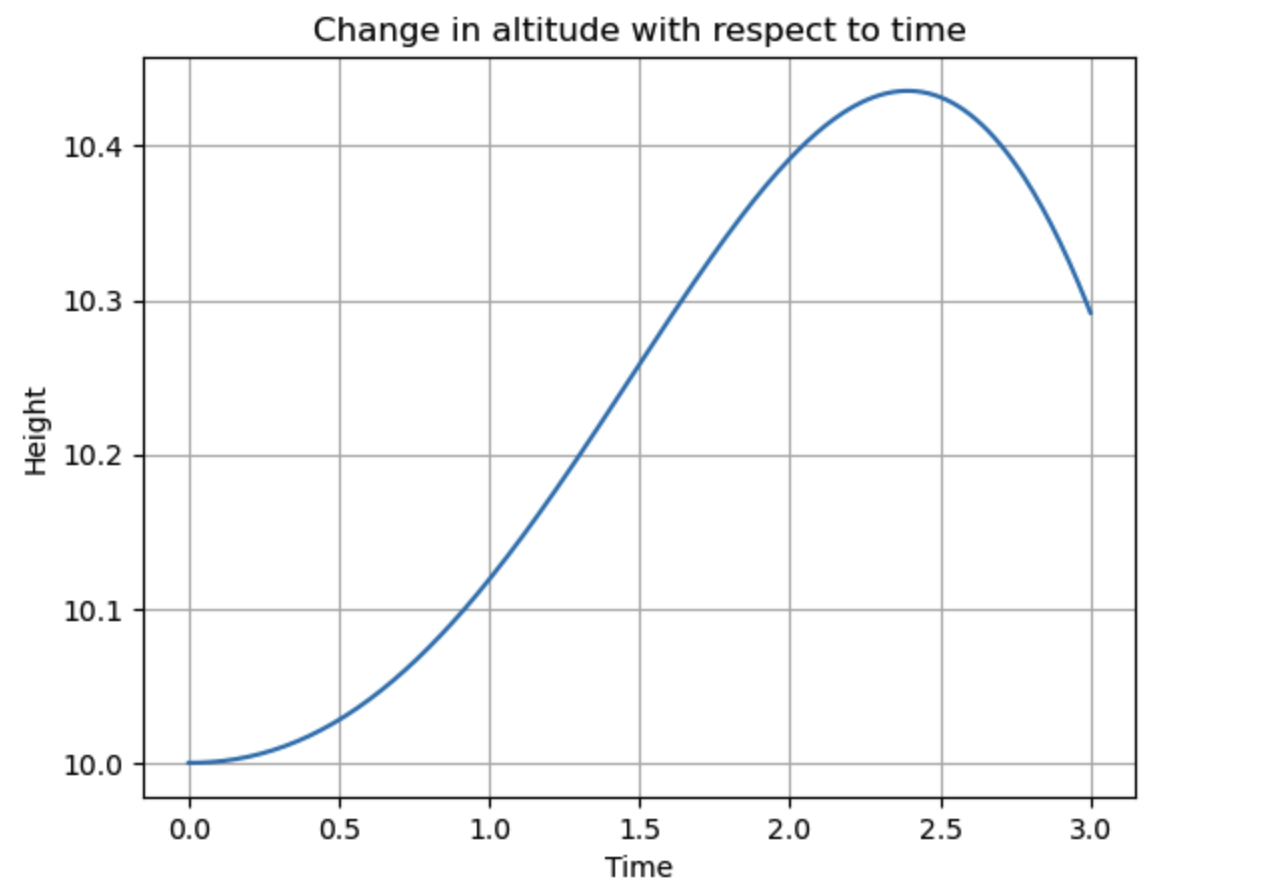
\includegraphics[width=0.5\textwidth]{image5.png}
    \label{fig:enter-label}
\end{figure}

\section{Part2-3 Height Controller}

In the conducted simulation, the PD controller was tasked to compensate for a known discrepancy between the assumed and actual mass of the robot. The controller was designed for an assumed mass (\( \hat{m} \)) of 1.0 unit, while the actual mass (\( m \)) was 0.8 units. This mass mismatch poses a significant challenge for the controller's ability to achieve precise height control.

The `simulate\_with\_mass` function was appropriately modified to utilize the actual mass in calculating the robot's acceleration. The control inputs, derived from the PD controller, were scaled accordingly to ensure that the actual dynamics of the robot were accurately represented in the simulation.

Despite the adjustments made for the actual mass, the PD controller, with its gains tuned for the assumed mass, applied a force that led to an overshoot in the robot's altitude. The following plot illustrates the trajectory of the robot's height over time in comparison to the desired height.

As evidenced by the simulation results, the robot was able to reach and exceed the desired height, but could not maintain it due to the excessive force exerted by the controller. This result highlights the need for controllers that can adapt to parameter uncertainties or systems that can accurately identify and compensate for such discrepancies.

\begin{figure}[htbp]
    \centering
    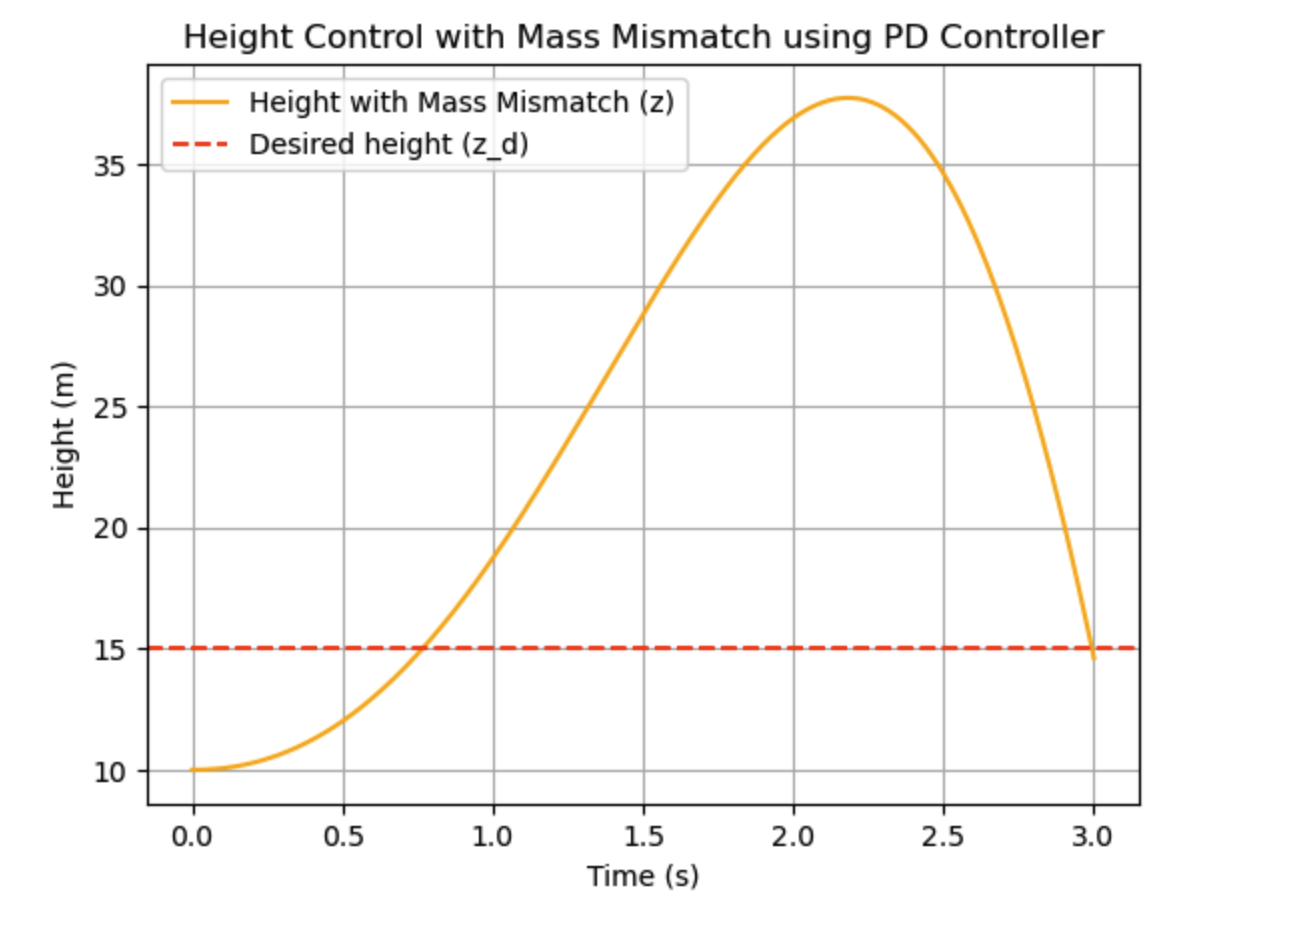
\includegraphics[width=0.5\textwidth]{image6.png}
    \label{fig:enter-label}
\end{figure}

\end{document}
